\chapter{Modelo escogido y entorno de trabajo}

Una vez disponemos de los conjuntos de datos seleccionados, y establecidos los métodos de codificación que queremos probar, podemos pasar a la construcción del entorno de trabajo. De por sí solos, los métodos de encoding no puede ser evaluados, ya que requieren su aplicación en un modelo concreto que lo acepte de entrada y sea capaz de procesarlo y aprender del embedding proporcionado.\\

En la sección del estado del arte (capítulo \ref{sota}), estudiamos multitud de modelos basados en Transformers que podríamos usar como base para nuestras pruebas. Sin embargo, en varios de los casos, los mecanismos de atención eran muy elaborados, y podrían dificultar apreciar el impacto del positional encoding evaluado. Por ello, para su evaluación, se ha optado por tomar una base similar a Informer, que nos permitirá encontrar un equilibrio entre un modelo adaptado a series temporales y un modelo lo suficientemente simple para ser comprendido y modificado.\\

Durante este apartado, analizaremos el funcionamiento del modelo adaptado, así como las cuestiones relativas al uso de los datos para realizar el entrenamiento, las cuales varían con respecto a un problema habitual.

\section{Modelo seleccionado: Informer}

El modelo seleccionado sobre el que evaluar el conjunto de datos es un elemento clave a la hora de medir el rendimiento de los mismos. En la actualidad, podemos encontrar una gran variedad de modelos, algunos más sofisticados y otros más sencillos, que aplican multitud de operaciones y tratan de extraer el mayor rendimiento posible del conjunto de datos. En este caso, deseamos un modelo que sea capaz de adaptarse correctamente a la estructura de una serie temporal, pero que además mantenga intacto el concepto de Transformer, que es el entorno de trabajo en el cual operamos mediante el enriquecimiento del encoding. Si bien podríamos operar con modelos que no utilizan atención, esta decisión podría dificultar medir el impacto real del encoding de los resultados, ya que en modelos ya vistos como Autoformer, la codificación está implícita dentro de la propia arquitectura mediante la autocorrelación, y resulta más complejo apreciar el impacto del encoding, o probar el caso extremo de suprimirlo completamente para obtener nuestro baseline.\\

Por estos motivos, se ha optado por hacer uso de un modelo muy conocido y comparado en el estado del arte como es \textit{Informer}. Recordando su arquitectura de definición, este modelo destacaba por el uso de ProbSparse attention para reducir el coste del cómputo de atención a $O(n \log{n})$, empleaba el método de \textit{distillation} para reducir el tamaño de entrada de cada capa del encoder/decoder, y usaba un decoder estilo generador que permite simplificar el proceso de inferencia y predicción. Sin embargo, existe un aspecto clave que podría entrar en conflicto con nuestro problema el uso de ProbSparse.\\

Tal y como estudiamos en el apartado de estado del arte, \textit{ProbSparse} conseguía reducir el tamaño del producto realizado en atención realizando un muestreo mediante una distribución logarítmica de los tokens de entrada, con la teoría de escoger únicamente aquellos realmente representativos en el problema, y sustituyendo el resto por un valor medio predefinido que reduzca el número de operaciones.\\
	
Desde el punto de vista computacional, este proceso puede ser interesante y útil para reducir la complejidad del problema considerado, pero está afectando negativamente al desempeño de la codificación: en caso de usar encodings que favorezcan el contexto local, como nuestro caso mediante el uso de la ventana, o métodos semánticos como TPE, suprimir valores estimados como de ``escaso valor'' podría realmente estar eliminando puntos esenciales para estas codificaciones, y romper la localidad de los datos, tal y como otras propuestas vistas han detectado.\\

De este modo, el uso de los PE podría verse gravemente afectado. Desde una perspectiva crítica, el mecanismo \textit{ProbSparse} podría resultar perjudicial para la preservación de la semántica de los datos. Como alternativa, se ha optado por emplear la definición original del Transformer que, aunque presenta una complejidad cuadrática $O(n^2)$, permite evaluar la efectividad real de nuestras propuestas sin comprometer la coherencia semántica.\\

Con esta configuración, basada en el comportamiento tradicional de los Transformers, se dispone de un entorno de comparación justo, libre de operaciones adicionales que puedan distorsionar los resultados o dificultar su análisis, haciendo posible estudiar variables como el impacto del \textit{encoding} frente a la secuencia, y establecer comparaciones con el modelo original de codificación posicional de la forma más directa posible.

\section{Particionado y procesado de los datos}

Otro de los aspectos claves que configuran el entorno de experimentación es el particionado de los datos para la posterior evaluación de rendimiento. En este punto, estudiaremos la importancia de un correcto particionado de los datos, teniendo especial cuidado en respetar la estructura propia de las series temporales, y analizando la importancia de disponer de un estimador no sesgado del modelo
entrenado. Finalmente, definiremos la estrategia a seguir.

\subsection{Importancia de la separación train-test}

En cualquier tarea de aprendizaje, ya sea aprendizaje automático tradicional, deep learning, o en nuestro caso, Transformers para series temporales, disponer del mayor número de datos posible es el objetivo deseable, ya que aunque aumentan el coste del experimento, nos ofrecen unos resultados más fieles al fenómeno real que queremos modelar.\\

Sin embargo, cuando realizamos un modelo de aprendizaje, realmente estamos creando una hipótesis: procedemos a la selección de un modelo concreto de entre un conjunto de estos, con el objetivo de que su resultado se acerque lo máximo posible al comportamiento real del problema, el cual está modelado a través de una función $f$ que desconocemos. Pero, para poder estimar la bondad de nuestro ajuste de forma fiable, necesitamos algún estimador no sesgado que nos refleje la calidad del modelo escogido y nos permita saber el error que comete nuestra hipótesis con respecto a la distribución de la población real, $E_{out}$. Cuando construimos un modelo, estamos empleando una muestra de la población, la cual es recorrida continuamente durante el proceso de entrenamiento para ir ajustando los filtros aplicados sobre el conjunto y que permite inferir el comportamiento del fenómeno modelo empleando métodos de gradiente, y en definitiva, fuerza bruta.\\

Por tanto, buscamos conseguir un estimador no sesgado, separando un conjunto de datos del total, y obteniendo un conjunto de test, el cual no se haya visto involucrado en ninguna fase del proceso de aprendizaje. La hipótesis final, a la que llamaremos $g$, es evaluada en este subconjunto, y el resultado será un buen estimador del $E_{out}$. Normalmente, a este error se le denomina $E_{test}$, y al seleccionarlo como estimador de $E_{out}$, estamos afirmando de alguna manera de que éste se tratará de un estimador que generaliza muy bien el error fuera de la muestra.\\

Este conjunto recibirá un número efectivo de hipótesis $|\mathcal H|= 1$, es decir, solamente se evaluará con el ajuste final realizado por el modelo, una vez finaliza su ajuste. Por tanto, la hipótesis se elige sin conocer el comportamiento de los datos que el conjunto de test contiene, ya que si la estimación de $g$ se viese afectada por instancias de entrenamiento estaríamos sesgando el resultado, y la ecuación de Hoeffding, la cual respalda esta teoría, no será aplicable. Dicha ecuación enuncia, que para muestras idénticamente distribuidas, e independientes entre sí, se cumple la desigualdad \ref{eqn:hoeffding}.

\begin{equation}
	\label{eqn:hoeffding}
	\centering 
	P(\mathcal{D}: | E_{out}(h) E_{in}(h) |  > \epsilon \leq 2e^{-2\epsilon^2	N}
\end{equation}


Donde, para cualquier valor de $\epsilon$:
\begin{itemize}
	\item $\mathcal{D}$ es el nombre que recibe el conjunto de entrenamiento.
	\item $ E_{out}$ es el error out-of-sample, error teórico con respecto a distribución real de los datos.
	\item  $E_{in}$ es el error in-sample, es decir, el error cometido durante el proceso de entrenamiento entre las etiquetas inferidas, y su valor real, también conocido como $y$ verdadero.
	\item $N$ es el tamaño de la muestra de datos disponible.
\end{itemize}

Es decir, se cumple que $E_{out}$ resulta una estimación fiable del modelo. El valor del entrenamiento, $E_{in}$, sí que sería un estimador sesgado de manera optimista, pues dicho conjunto ha sido sometido al proceso de ajuste continuamente, y ha determinado la distribución final de pesos del modelo, por lo que quedarnos con su valor como estimación, sobre todo con arquitecturas tan profundas y potentes a nivel de cálculo como los Transformers, sería un grave error.\\

Mantener un equilibrio para la proporción de la partición es clave; a mayor tamaño de la partición de test, más cercano será el valor de $E_{test}$ con respecto a $E_{out}$. Pero, cuantos menos datos para entrenar dispongamos, peor será la estimación al comportamiento real de la población $f$. Normalmente, los valores recomendados suelen ser entre un 10\%-30\% de porcentaje de los datos dedicados al conjunto de test, quedando entre un 70 \%-90\% de datos de entrenamiento.\\

Pero, debemos tener especial cuidado en nuestro contexto. Para el cumplimiento de la desigualdad, las restricciones de independencia y pertenencia a la misma distribución son claves, por lo que una correcta separación de ambos conjuntos es esencial. En series temporales, la estructura secuencial de los datos supone una condición indispensable a mantener para no perjudicar la semántica del problema y obtener resultados coherentes, ya que una de las principales diferencias de una serie temporal con respecto a un conjunto tabular tradicional es la dependencia de cada valor con los anteriores (el orden). Por tanto, realizar separaciones estocásticas del conjunto de datos para obtener las particiones de entrenamiento y test es inviable, y debemos realizar separaciones en las que se mantenga la secuencialidad original.\\

 Una estrategia simple y efectiva por la que se suele optar es la separación de tipo \textit{last-block}, en la que se extrae secuencialmente la parte final de la secuencia temporal para construir test, pero asegurándonos de no tomar algunas de las posiciones entorno al punto de separación, ya que estaríamos sesgando el resultado al incorporando contexto altamente correlado. En nuestro caso, siguiendo el consejo, una partición del 70-30 resulta más que suficiente, y será la proporción escogida para los datasets anteriormente seleccionados.\\
 
 Pero, aún nos resta realizar una segunda división, necesaria para el correcto ajuste del modelo: la partición de validación, una partición ligeramente más sesgada que test, pero que nos permitirá evaluar el rendimiento del modelo al final de cada época. En el siguiente punto, analizaremos su importancia y las diferentes estrategias.

\subsection{Partición de validación. Estrategias de división para series temporales}

Hasta este punto, disponemos de dos particiones de datos, train y test, siendo esta última reservada para la evaluación final de nuestra hipótesis. Por tanto, desde este punto, únicamente podremos operar con el conjunto de entrenamiento, y debemos realizar un uso adecuado que nos permita medir la mejora de rendimiento en cada época del proceso de entrenamiento, y facilite la elección de parámetros y la detección de posibles fenómenos como el sobreaprendizaje.\\

La forma más sencilla de lograrlo es mediante el ya nombrado conjunto de validación. Este es similar al conjunto de test, pero como principal diferencia de uso, es extraído del conjunto de entrenamiento y se usa para evaluar el correcto ajuste del modelo y el rendimiento de los parámetros elegidos. Matemáticamente, el error asociado a esta partición, $E_{val}$, actúa como estimador directo del error \textit{out-of-sample}, ya que se calcula evaluando el modelo sobre los $K$ valores reservados para validación y que no se han utilizado durante el entrenamiento, tal y como se muestra en la ecuación \ref{eqn:equiv}.

\begin{equation}
	\label{eqn:equiv}
	\centering
	E_{out}(g) \approx E_{out}(g^-) \approx E_{val}(g^-)
\end{equation}


Siendo $E_{out}(g)$ el error final cuando se utiliza todo el conjunto de datos $\mathcal D$.\\

La parte izquierda de la ecuación funciona mejor cuanto más pequeña sea k, mientras que por la derecha, un mayor valor de k permitirá una mejor estimación a través de $E_{val}$. El caso ideal sería, para acercarnos lo máximo posible entre $E_{out}(g)$ y $ E_{out}(g^-)$, elegir k lo más pequeño posible, cuyo caso extremo es k=1, pero esto no sería viable. Normalmente, se suelen optar por alternativas como validación cruzada de $v$ folds, donde los datos se dividen en k particiones, y el conjunto de validación rota por cada una de ellas, obteniendo $E_{val}$ como la media de los $v$ errores parciales. Sin embargo, normalmente su construcción se hace mediante un particionado aleatorio en $v$ conjuntos, rompiendo una vez más la condición estructural de las series temporales. Por lo tanto, en el estado del arte~\cite{bergmeir2012use} podemos encontrar varias alternativas (ver figura \ref{valid}):

\begin{itemize}
	\item \textbf{Validación cruzada ordenada}. Consiste en realizar el proceso de sondeo de manera aleatoria, pero respetando el orden de las instancias escogidas, es decir, ordenando por timestamp. De esta forma, si bien las diferentes muestras pueden estar distanciadas entre sí, respetan al menos el orden temporal. Realmente, no es un método especialmente deseable, ya que tomar valores aislados podría introducir sesgos al estimador al poder ser fácilmente obtenidos de su entorno. Se deberían suprimir el entorno para evitar esta problemática.
	\item \textbf{Validación cruzada no dependiente}. Propone una solución simple al problema de las dependencias visto en la CV estándar: eliminar los valores cercanos a los puntos seleccionados. Sin embargo, esto supone una gran pérdida de información útil.
	\item \textbf{Validación cruzada por bloques}. Para evitar la pérdida excesiva de información que resulta al eliminar valores dependientes aislados, se realiza la propuesta de seleccionar, en lugar de valores únicos, bloques completos, de forma que sólo sea necesario eliminar el contexto de antes y después de cada bloque. Conseguimos así conjuntos de observaciones contiguas, respetando el orden temporal y permitiendo estimaciones más robustas aprovechando mejor la información.
	\item \textbf{Last-block / particionado tradicional}. Es el particionado tradicional, en el que se escoge el último conjunto de valores eliminando el contexto cercano con el resto del conjunto de entrenamiento. Es la estrategia ya seguida al realizar la partición train-test.
\end{itemize}

\begin{figure}[!ht]
	\centering
	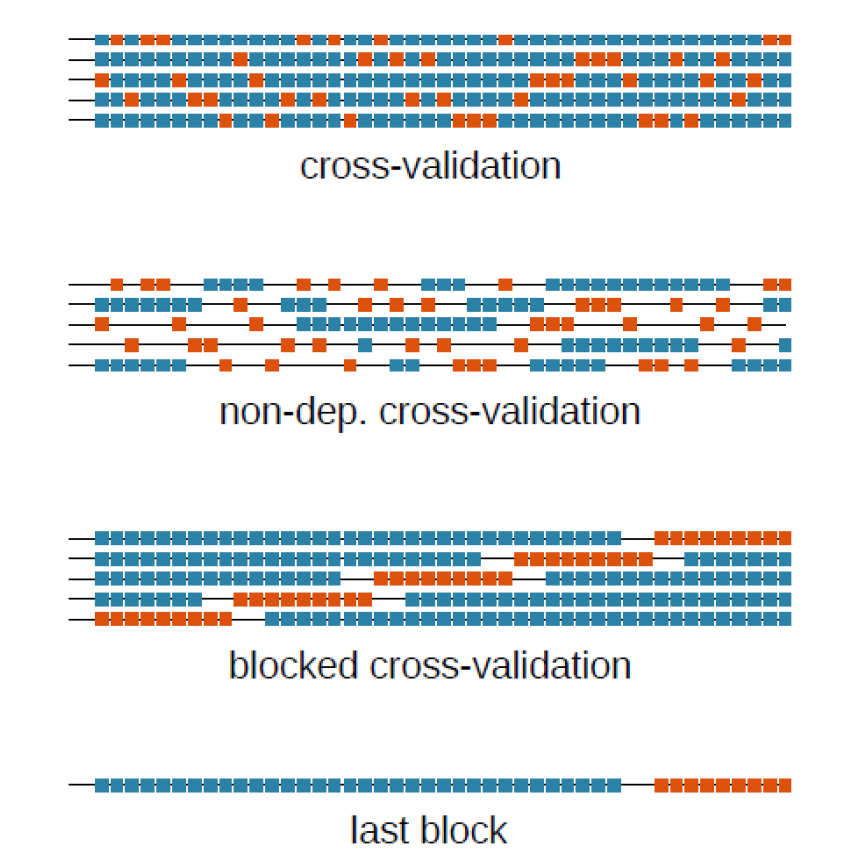
\includegraphics[scale=0.35]{img/valid}
	\caption{Partición de datos: estrategias de validación cruzada en series temporales \cite{bergmeir2012use}}
	\label{valid}
\end{figure}


Si bien, experimentalmente la opción de validación por bloques (originalmente \textit{Blocked Cross-validation}) ofrece buenos resultados experimentalmente, ha de cumplir algunas restricciones, como cumplir el principio de estacionariedad. Esta limitación, unida a la necesidad de reentrenar el modelo tantas veces como bloques de validación se definan, implica un elevado coste computacional, agravado por el gran número de parámetros del modelo y la considerable longitud de los datos. Por este motivo, en los experimentos que se presentan a continuación se empleará nuevamente el criterio \textit{last-block} para la obtención del conjunto de validación, considerando las condiciones previamente mencionadas acerca de la necesidad de eliminar el contexto inmediato compartido con el conjunto de entrenamiento.

\section{Función de pérdida y métricas}

Cuando entrenamos el modelo, obtenemos una hipótesis final, la cual nos permitirá modelar una aproximación del conjunto de test, de manera que podremos comparar y evaluar la calidad del modelo con respecto a dichos datos. Pero, también necesitamos una referencia durante el entrenamiento que nos permita, de forma sencilla, comprender si el entrenamiento evoluciona favorablemente. El objetivo es simple: que dichos valores sean lo más cercano a cero, lo que se traduce como condición deseable que tanto $E_{in}$ como $E_{val}$ tiendan a cero.\\

En el caso de las series temporales, las funciones de evaluación empleadas coinciden con las utilizadas en problemas de regresión, dado que el objetivo es cuantificar el error continuo entre los valores predichos y los valores reales a lo largo de toda la secuencia temporal. Este enfoque se justifica porque la predicción de series temporales implica estimar variables continuas en función del tiempo, lo que la enmarca formalmente como un problema de regresión, pero en el dominio temporal.\\

En este trabajo, emplearemos principalmente las métricas \textit{Mean Absolute Error} (MAE) y \textit{Mean Squared Error} (MSE) para la comparación de resultados,  mientras que en el caso de función de pérdida usaremos MSE. No obstante, también se incluye el cálculo de otras métricas complementarias, tales como \textit{Mean Absolute Percentage Error} (MAPE), \textit{Mean Squared Percentage Error} (MSPE) y \textit{Root Mean Squared Error Mean} (RMSE\_Mean), cuyo funcionamiento es bastante similar a dos anteriores pero nos permiten tener una visión más completa del rendimiento de los modelos evaluados:

\begin{itemize}
	\item \textbf{MSE}. Es la función de pérdida para regresión por excelencia, así como una adecuada métrica de rendimiento, debido a su simplicidad de cálculo y a que su formulación cuadrática permite un tratamiento analítico mediante técnicas de cálculo diferencial, Mide la distancia de cada punto real de la serie hasta el valor estimado, de forma que se penaliza por cada punto de forma equivalente a la magnitud de esa distancia. Se puede expresar como:
	
	$$\mathrm{MSE} = \frac{1}{n} \sum_{i=1}^n (y_i - \hat{y}_i)^2$$ 
	
	donde \(y_i\) es el valor observado, \(\hat{y}_i\) es el valor predicho y \(n\) es el número de observaciones.  
	
	
	\item \textbf{MAE}. Es una métrica bastante similar al MSE. Calcula el error entre cada par de puntos real y estimado, pero se basa en realizar la diferencia entre el valor actual y la predicción del error para un punto dado:
	$$abs(y_i - \lambda (x_i))$$
	
	Estos errores posteriormente son sumados para quedarnos con su valor medio, y así obtener la distancia promedio:
	$$\mathrm{MAE} = \frac{1}{n} \sum_{i=1}^n \left| y_i - \hat{y}_i \right|$$
	
	
	\item \textbf{MAPE}. Expresa el error promedio de la estimación en términos relativos, expresándolo como un porcentaje respecto al valor real de cada observación. Al ser un valor en porcentaje, nos permite obtener una tasa de error normalizada. Sin embargo, debemos tener especial cuidado con los valores cercanos a cero, ya que los errores en dichos valores pueden inflar artificialmente el porcentaje de error. En nuestro caso, al tener mediciones normalizadas, y valores muy pequeños, su uso podría ser arriesgado, y es por eso que se optó finalmente por usar MSE para la función de pérdida.
	
	$$
	\mathrm{MAPE} = \frac{100}{n} \sum_{i=1}^n \left| \frac{y_i - \hat{y}_i}{y_i} \right|
	$$
	
	
	\item \textbf{MSPE}. Puede entender como la versión cuadrática del MAPE, la cual penaliza de manera más severa los errores relativos grandes al elevar al cuadrado los errores relativos. De esta forma, se potencia la influencia de predicciones que se alejan significativamente del valor real. Al igual que MAPE, permite comparar errores entre series de diferentes escalas, pero también comparte la inestabilidad frente a valores cercanos a cero. Se define como:
	
	$$
	\mathrm{MSPE} = \frac{100}{n} \sum_{i=1}^n \left( \frac{y_i - \hat{y}_i}{y_i} \right)^2
	$$
	
	\item \textbf{RMSE}. Es la raíz cuadrada del MSE. A diferencia del MAE, RMSE penaliza más fuertemente los errores grandes debido a la elevación al cuadrado, lo que lo hace útil cuando se quieren evitar grandes desviaciones. Sin embargo, esta misma característica lo hace más sensible a valores atípicos, por lo que si bien es útil a nivel informativo, puede ser crítica si se usa en series temporales, donde esto es uin fenómeno frecuente. Su expresión es:
	$$
	\mathrm{RMSE} = \sqrt{\frac{1}{n} \sum_{i=1}^n (y_i - \hat{y}_i)^2}
	$$
\end{itemize}

En conjunto, con estas 5 métricas disponemos de una buena variedad de resultados que nos permitirán supervisar el resultado y comparar entre alternativas adecuadamente.


\section{Framework de trabajo y especificaciones hardware}

La realización de todo el proceso experimental se realizará haciendo uso de Python~\footnote{Python: \url{https://www.python.org/}}, debido a la gran acogida del lenguaje en el ámbito de la inteligencia artificial, llegando incluso a desplazar a R como principal lenguaje empleado en las publicaciones académicas recientes. Para el desarrollo del trabajo, emplearemos multitud de librerías que facilitan el procesado de datos, pero de entre todas ellas destaca Pytorch~\cite{paszke2019pytorchimperativestylehighperformance}.\\

Su elección viene motivada por su tendencia creciente en las publicaciones científicas, así como su interfaz simplificada frente a TensorFlow. Aunque ambas soluciones nos otorgan funcionalidades equivalentes, las cuales son cada vez más accesibles gracias a diferentes API externas de alto nivel, Pytorch ofrecía un mejor equilibrio entre la baja granularidad de implementación, y el uso de bloques funcionales con los que construir y editar modelos sin entrar en detalles de bajo nivel, como la implementación de las métricas, las capas totalmente conectadas o las convoluciones. Además, el modelo empleado como base, Informer, dispone de una implementación funcional en GitHub~\cite{zhouhaoyi2020informer} realizada en este entorno.\\

En cuanto al preprocesado de los datos, se han empleado las siguientes librerías: NumPy~\cite{harris2020array} para la vectorización de operaciones; Pandas~\cite{mckinney-proc-scipy-2010} para la lectura y transformación de los ficheros \textit{.csv} y \textit{.parquet}; y Matplotlib~\cite{Hunter:2007} y statmodels~\cite{seabold2010statsmodels} para representaciones gráficas y análisis previo de los datos.\\

La ejecución de todos los experimentos se ha realizado haciendo uso del clúster DGX, propiedad de la Universidad de Granada, debido a la necesidad de recursos de cómputo abundantes para la ejecución de cada variante. Los recursos empleados para cada ejecución han sido:

\begin{itemize}
	\item Procesador: x 32 cores Intel® Xeon® E5-2698.
	\item RAM: 96GB
	\item GPU: x 1 Tesla V100 32GB 
\end{itemize}

Para garantizar la estabilidad numérica y la reproducibilidad de los resultados, todos los experimentos se han ejecutado múltiples veces utilizando una semilla aleatoria. Esta práctica permite reducir impacto propio de la inicialización aleatoria de los modelos y al muestreo de datos, asegurando que los resultados reflejen de manera más fiel el comportamiento real del modelo. En particular, se realizaron tres iteraciones independientes para cada configuración experimental, calculando posteriormente el promedio estadístico de cada una de las métricas y suavizar el impacto de ejecuciones atípicas o fluctuaciones aleatorias.\\

La ejecución de los experimentos se realiza mediante el script \texttt{run\_exp.py}, disponible en el repositorio del TFM\footnote{Repositorio: \url{https://github.com/hexecoded/tfm}}. Este script permite configurar de manera flexible el modelo mediante numerosos parámetros de entrada, incluyendo la selección de los distintos tipos de codificación posicional y sus hiperparámetros asociados.

